% Slide 37: Proximity Measures
\begin{frame}{معیارهای مجاورت: شباهت و فاصله}{\lr{Proximity Measures: Similarity \& Distance}}
  \begin{itemize}
    \setlength{\itemsep}{6pt}
    \item تا اینجا الگوریتم‌های مختلف خوشه‌بندی را بررسی کردیم؛ \textbf{همه این روش‌ها به معیارهای مجاورت وابسته هستند}.
    \item \textbf{شباهت:} \lr{(Similarity)}
    \begin{itemize}
      \setlength{\itemsep}{3pt}
      \item یک معیار عددی برای سنجش میزان همسانی دو شیء داده (مقدار بالاتر $\Rightarrow$ شباهت بیشتر).
      \item معمولاً در بازه $[0, 1]$ نرمال‌سازی می‌شود.
    \end{itemize}
    \item \textbf{عدم‌شباهت یا فاصله:} \lr{(Dissimilarity / Distance)}
    \begin{itemize}
      \setlength{\itemsep}{3pt}
      \item یک معیار عددی برای سنجش میزان تفاوت دو شیء داده (مقدار بالاتر $\Rightarrow$ تفاوت بیشتر).
      \item حداقل عدم‌شباهت برابر با $0$ است (تطابق کامل).
      \item حد بالای فاصله بسته به نوع تابع متغیر است.
    \end{itemize}
    \item انتخاب معیار مناسب کاملاً به ماهیت داده‌ها و الزامات کاربرد بستگی دارد.
  \end{itemize}
\end{frame}

% Slide 38: Proximity of Single Attributes
\begin{frame}{مجاورت در ویژگی‌های تک‌متغیره}{\lr{Proximity of Single Attributes}}
  \begin{center}
    {\fontsize{9}{11}\selectfont\color{mannheimblue}\textbf{فرمول‌های محاسبه شباهت ($s$) و عدم‌شباهت ($d$) برای مقادیر $p$ و $q$}}\\[0.2cm]
    \resizebox{\textwidth}{!}{%
    \begin{tabular}{|l|c|c|}
      \hline
      \textbf{نوع ویژگی \lr{(Attribute Type)}} & \textbf{عدم‌شباهت \lr{(Dissimilarity)} $d$} & \textbf{شباهت \lr{(Similarity)} $s$} \\
      \hline
      \textbf{اسمی \lr{(Nominal)}} & 
      $d = \begin{cases} 0 & p = q \\ 1 & p \neq q \end{cases}$ & 
      $s = \begin{cases} 1 & p = q \\ 0 & p \neq q \end{cases}$ \\
      \hline
      \textbf{ترتیبی \lr{(Ordinal)}} & 
      $d = \frac{|p - q|}{n - 1} \quad (0 \le p,q \le n-1)$ & 
      $s = 1 - \frac{|p - q|}{n - 1}$ \\
      \hline
      \textbf{فاصله‌ای / نسبتی \lr{(Interval / Ratio)}} & 
      $d = |p - q|$ & 
      $s = -d \quad \text{یا} \quad s = \frac{1}{1 + d} \quad \text{یا} \quad s = 1 - \frac{d - \min(d)}{\max(d) - \min(d)}$ \\
      \hline
    \end{tabular}%
    }
  \end{center}
\end{frame}

% Slide 39: Levenshtein Distance
\begin{frame}{فاصله لونشتاین برای رشته‌ها}{\lr{Levenshtein Distance for Strings}}
  \begin{itemize}
    \setlength{\itemsep}{5pt}
    \item معیاری برای اندازه‌گیری \textbf{عدم‌شباهت دو رشته متنی} \lr{(String Dissimilarity)}.
    \item برابر با \textbf{حداقل تعداد عملیات ویرایشی} لازم برای تبدیل یک رشته به رشته دیگر.
    \item \textbf{عملیات ویرایشی مجاز:}
    \begin{itemize}
      \setlength{\itemsep}{2pt}
      \item درج یک نویسه \lr{(Insertion)}.
      \item حذف یک نویسه \lr{(Deletion)}.
      \item جایگزینی یک نویسه با نویسه دیگر \lr{(Substitution)}.
    \end{itemize}
    \item \textbf{مثال‌ها:}
    \begin{itemize}
      \setlength{\itemsep}{2pt}
      \item $\text{levenshtein}(\text{'table'}, \text{'cable'}) = 1$ \ \lr{(1 substitution)}
      \item $\text{levenshtein}(\text{'Doe, Jane'}, \text{'Jane Doe'}) = 8$ \ \lr{(7 substitutions, 1 deletion)}
    \end{itemize}
  \end{itemize}
\end{frame}

% Slide 40: Further String Similarity Measures
\begin{frame}{سایر معیارهای شباهت رشته‌ها}{\lr{Further String Similarity Measures}}
  \begin{columns}[T]
    \begin{column}{0.48\textwidth}
      \textbf{دسته‌بندی معیارهای متنی:}
      \begin{itemize}
        \setlength{\itemsep}{4pt}
        \item \textbf{مبتنی بر ویرایش:} \lr{(Edit-based)} لونشتاین، همینگ، \lr{Jaro-Winkler}.
        \item \textbf{مبتنی بر توکن / کلمه:} \lr{(Token-based)} ژاکارد \lr{(Jaccard)}، کسینوسی \lr{(Cosine)}.
        \item \textbf{آوایی:} \lr{(Phonetic)} \lr{Soundex} و تلفظ صوتی.
        \item \textbf{ترکیبی و تعبیه‌محور:} \lr{(Embedding)} مدل‌های \lr{fastText} و \lr{BERT}.
      \end{itemize}
      {\scriptsize\color{subgray} (موضوع تخصصی درس یکپارچه‌سازی داده‌های وب)}
    \end{column}
    \begin{column}{0.5\textwidth}
      \begin{center}
        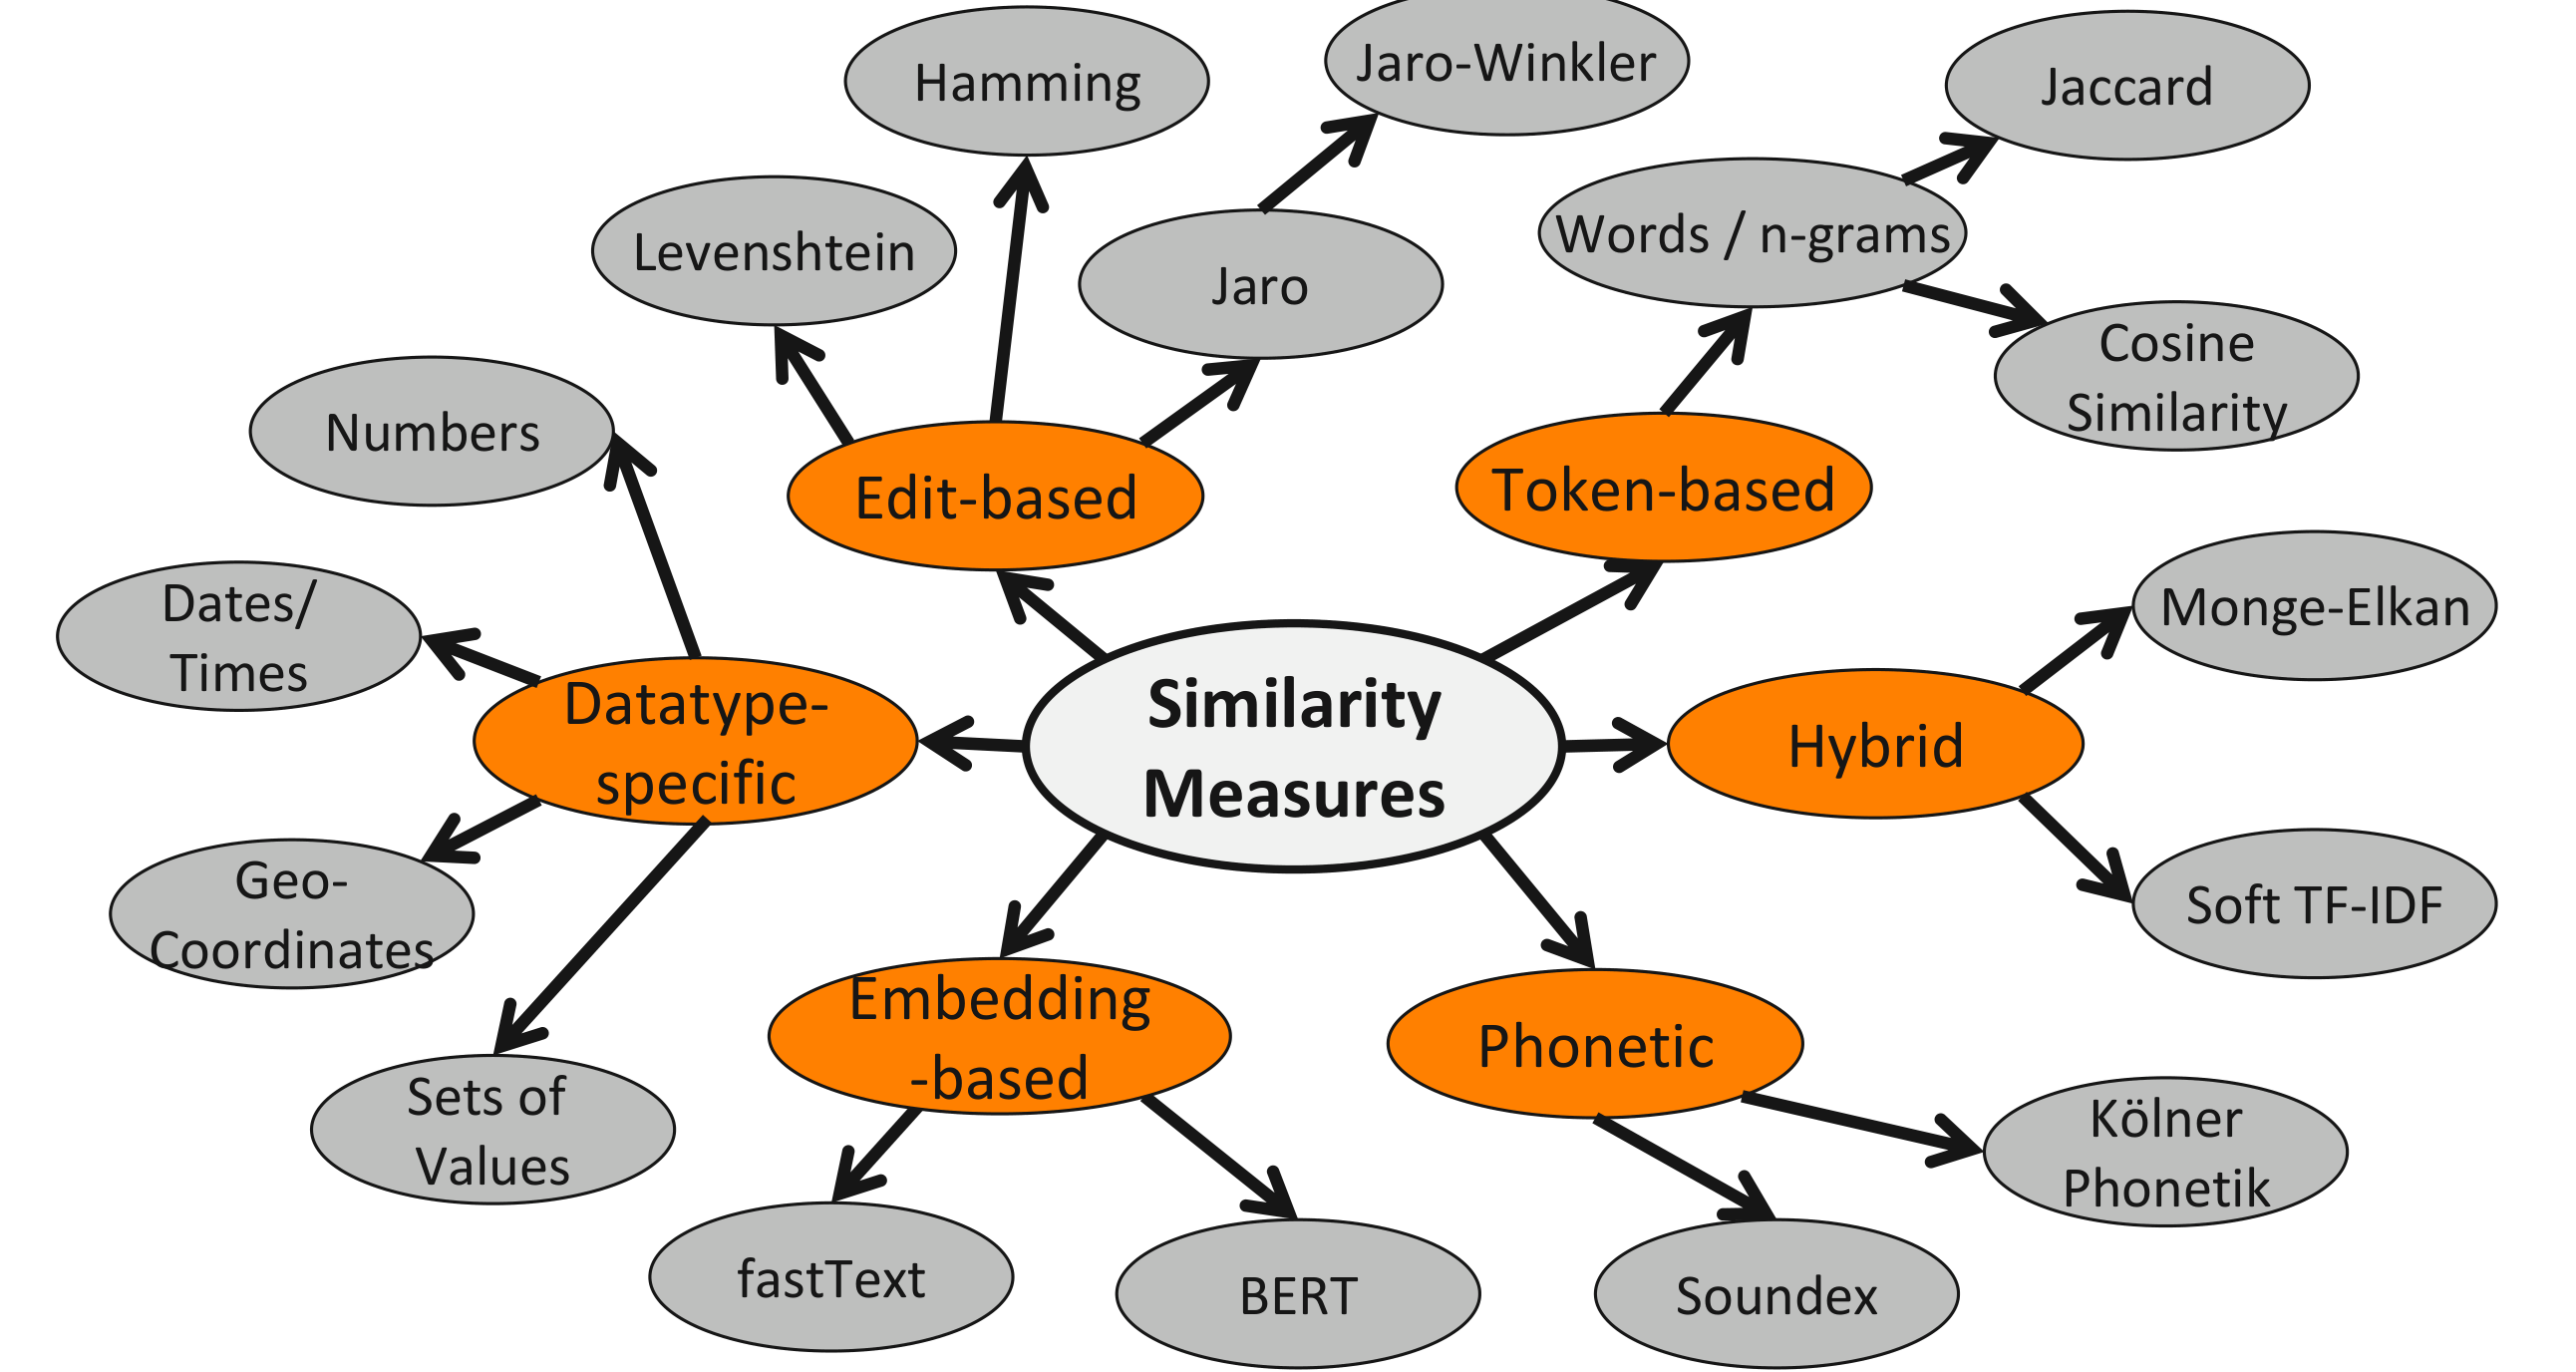
\includegraphics[width=\textwidth,height=4.6cm,keepaspectratio]{images/slide40_string_similarity.png}
      \end{center}
    \end{column}
  \end{columns}
\end{frame}

% Slide 41: Proximity of Multidimensional Data Points
\begin{frame}{مجاورت در نقاط داده چندبعدی}{\lr{Proximity of Multidimensional Data Points}}
  \begin{itemize}
    \setlength{\itemsep}{6pt}
    \item تا به اینجا معیارهای ارزیابی یک ویژگی منفرد را بررسی کردیم.
    \item اما در مسائل داده‌کاوی واقعی، رکوردها دارای \textbf{چندین بعد و ویژگی} هستند:
    \begin{itemize}
      \item مانند سن، قد، وزن، درآمد، سابقه و ...
    \end{itemize}
    \item بنابراین به معیارهای تجمیعی برای سنجش فاصله میان بردارها نیازمندیم.
    \item \textbf{نکته بسیار حیاتی: نرمال‌سازی \lr{(Normalization)}}
    \begin{itemize}
      \item ویژگی‌ها باید حتماً پیش از محاسبه فاصله نرمال‌سازی شوند (مانند $\text{Min-Max}$ یا $\text{Z-Score}$) تا متغیرهایی با مقیاس‌های عددی بزرگ‌تر بر کل فاصله غلبه نکنند و همه ویژگی‌ها وزن برابری داشته باشند.
    \end{itemize}
  \end{itemize}
\end{frame}

% Slide 42: Norms
\definecolor{l2green}{RGB}{0, 145, 65}
\definecolor{l1orange}{RGB}{215, 135, 0}
\begin{frame}{نُرم‌ها و فواصل مینکوفسکی}{\lr{Vector Norms \& Minkowski Distance}}
  \begin{columns}[T]
    \begin{column}{0.58\textwidth}
      {\fontsize{8.0}{10.5}\selectfont
      \begin{itemize}
        \setlength{\itemsep}{2pt}
        \item \textbf{\textcolor{l2green}{فاصله اقلیدسی}} \lr{($L_2$-norm)}
        \par\vspace{2pt}\noindent\makebox[\linewidth][c]{$\displaystyle \text{dist} = \sqrt{\sum_{k=1}^n (p_k - q_k)^2}$}\par\vspace{2pt}
        \item \textbf{حالت عمومی‌تر --- فاصله مینکوفسکی} \lr{($L_p$-norm)}
        \par\vspace{2pt}\noindent\makebox[\linewidth][c]{$\displaystyle \text{dist} = \sqrt[p]{\sum_{k=1}^n |p_k - q_k|^p} = \left(\sum_{k=1}^n |p_k - q_k|^p\right)^{\frac{1}{p}}$}\par\vspace{2pt}
        \item \textbf{\textcolor{l1orange}{فاصله منهتن}} \lr{($L_1$-norm)}
        \par\vspace{2pt}\noindent\makebox[\linewidth][c]{$\displaystyle \text{dist} = \sum_{k=1}^n |p_k - q_k|$}\par\vspace{1pt}
        \begin{itemize}
          \setlength{\itemsep}{1pt}
          \item کوتاه‌ترین مسیر میان دو تقاطع در شهر شطرنجی (منهتن یا مانهایم!).
        \end{itemize}
        \item {\fontsize{6.3}{7.5}\selectfont\color{subgray} ($n$: تعداد ابعاد؛ $p_k, q_k$: مقدار ویژگی $k$-ام نقاط داده $p$ و $q$)}
      \end{itemize}
      }
    \end{column}
    \begin{column}{0.40\textwidth}
      \begin{center}
        {\fontsize{8.5}{11}\selectfont
        \textbf{مثال عددی \lr{(Example)}}\\[0.1cm]
        \textcolor{l2green}{$\mathbf{L_2 = \sqrt{4^2 + 3^2} = 5}$}\\[0.05cm]
        \textcolor{l1orange}{$\mathbf{L_1 = 4 + 3 = 7}$}\\[0.15cm]
        }
        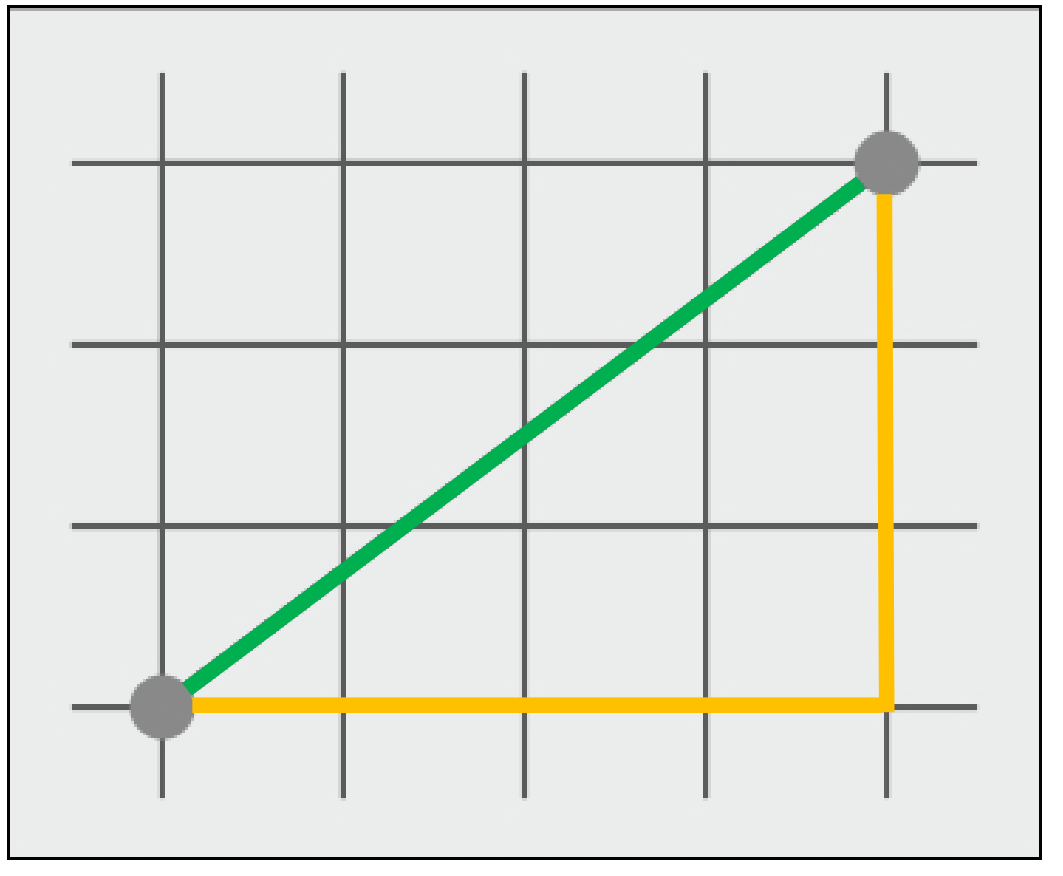
\includegraphics[width=0.92\textwidth,height=3.4cm,keepaspectratio]{images/slide42_norms_unit_shapes.png}
      \end{center}
    \end{column}
  \end{columns}
\end{frame}
